\documentclass[../main]{subfiles}
\begin{document}

\chapter{实现}%
\label{cha:realize}

\section{设计思路}%
\label{sec:design}

\begin{figure}[htpb]
  \centering
  \includegraphics[
    width = \linewidth,
  ]{dia}
  \caption{示意图}%
  \label{fig:dia}
\end{figure}

\begin{table}[htpb]
  \centering
  \caption{材料清单}%
  \label{tab:bom}
  \csvautobooktabular{tab/bom.csv}
\end{table}

\begin{figure}[htpb]
  \centering
  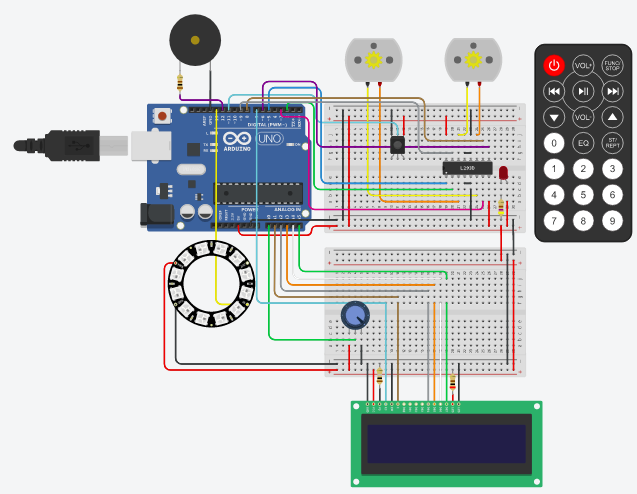
\includegraphics[
    width = 0.8\linewidth,
  ]{circuit}
  \caption{电路图}%
  \label{fig:circuit}
\end{figure}

\section{具体细节}%
\label{sec:detail}

\subsection{模拟信号源}%
\label{sub:analog}

可以用任何模拟信号源代替。但在仿真环境下,它们都等同于测量鼠标距离的电位器,
如图~\ref{fig:anaolog}。

\begin{figure}[htpb]
  \centering
  \begin{subfigure}[htbp]{0.28\linewidth}
    \centering
    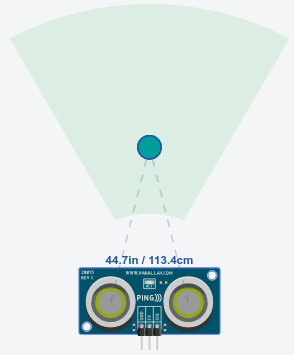
\includegraphics[
      width = \linewidth,
    ]{sensor/distance}
    \caption{距离传感器}%
    \label{fig:sensor/distance}
  \end{subfigure}
  \quad
  \begin{subfigure}[htbp]{0.28\linewidth}
    \centering
    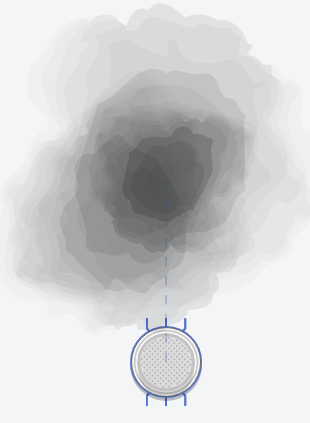
\includegraphics[
      width = \linewidth,
    ]{sensor/gas}
    \caption{气体传感器}%
    \label{fig:sensor/gas}
  \end{subfigure}

  \begin{subfigure}[htbp]{0.28\linewidth}
    \centering
    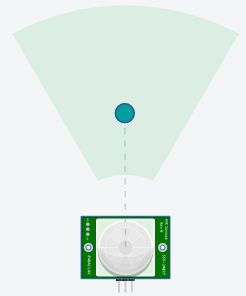
\includegraphics[
      width = \linewidth,
    ]{sensor/ir}
    \caption{红外传感器}%
    \label{fig:sensor/ir}
  \end{subfigure}
  \quad
  \begin{subfigure}[htbp]{0.28\linewidth}
    \centering
    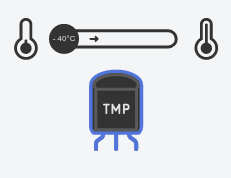
\includegraphics[
      width = \linewidth,
    ]{sensor/temparature}
    \caption{温度传感器}%
    \label{fig:sensor/temparature}
  \end{subfigure}

  \begin{subfigure}[htbp]{0.34\linewidth}
    \centering
    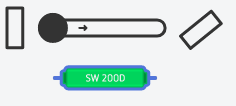
\includegraphics[
      width = \linewidth,
    ]{sensor/lean}
    \caption{斜度传感器}%
    \label{fig:sensor/lean}
  \end{subfigure}
  \caption{模拟信号源}%
  \label{fig:anaolog}
\end{figure}

ADC 采集到的数据经过式~\ref{eq:adc}换算得到结果——12连小彩灯点亮的个数。

\begin{align}
  \label{eq:adc}
  x = \frac{12x_0}{1023}
\end{align}

\subsection{控制设备}%
\label{sub:control}

在仿真环境下,控制设备们并不等同。

\subsubsection{LED灯}%
\label{ssub:led}

内部已经串联过电阻。选择的是可以显示3原色的12连小彩灯。模拟信号越强,亮的灯数
越多。

\subsubsection{蜂鸣器}%
\label{ssub:buzzer}

当模拟信号大于某一个阈值蜂鸣器响。

\subsubsection{电机}%
\label{ssub:motor}

L293D电机驱动原理如图~\ref{fig:l293d}。要保证相对的场效应管导通。

\begin{figure}[htpb]
  \centering
  \begin{subfigure}[htbp]{0.45\linewidth}
    \centering
    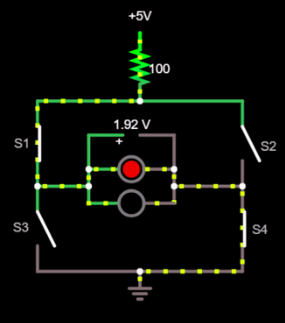
\includegraphics[
    width = \linewidth,
    ]{l293d/1}
    \caption{左}%
    \label{fig:l293d/1}
  \end{subfigure}
  \quad
  \begin{subfigure}[htbp]{0.45\linewidth}
    \centering
    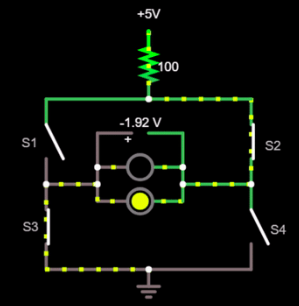
\includegraphics[
    width = \linewidth,
    ]{l293d/2}
    \caption{右}%
    \label{fig:l293d/2}
  \end{subfigure}
  \caption{H桥}%
  \label{fig:l293d}
\end{figure}

\subsubsection{串口}%
\label{ssub:serial}

波特率设置9600 。

\subsubsection{LCD显示屏}%
\label{ssub:lcd}

只有自带的ASCII 字库,实现中文需要得到相应点阵字模,如图~\ref{fig:dot}。

\begin{figure}[htpb]
  \centering
  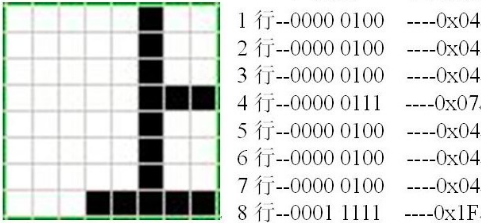
\includegraphics[
    width = 0.4\linewidth,
  ]{dot}
  \caption{点阵}%
  \label{fig:dot}
\end{figure}

网上大多数取字模软件的原理是利用了中国国标汉字库HZK, 这是一个二进制文件,包含
了中国所有汉字的点阵字模。其中HZK16,HZK24,HZK32分别对应了$16 \times 16, 24
\times 24, 32 \times 32$的点阵字模。只要输入一个汉字,就自动根据该字的区位码
找到在HZK中的点阵字模。但不幸的是LCD1602的每个字符是$5 \times 8$的。都不符合
我的要求。

于是如图~\ref{fig:dotfont}先把自己以前写的一个画画的程序\footnote{该程序的中
文介绍在 \href{https://zhuanlan.zhihu.com/p/141065072}{知乎专栏}。}改了改,按
快捷键修改颜色,灰色为0 ,黄色为1 ,蓝色是光标的位置。修改完后可以自动得到点
阵字模的值。如图 ~\ref{fig:dotfont}。原理是for循环读取每行的字符,将灰色和黄
色替换成0和 1,得到每行的一个01数组,再加权得到该行的字模。比如某行是01001, 那
么该行的字模用秦九韶算法是 $\Biggl(\biggl(\Bigl(\bigl((0 \times 2) + 1\bigr)
\times 2 + 0\Bigr) \times 2 + 0\biggr) \times 2 + 1\Biggr) \times 2 + 0$ ,用
级数法是 $\sum^{n}_{i = 0} a_i2^i$。可以利用同样的方法在显示屏上显示图形。

\begin{figure}[htpb]
  \centering
  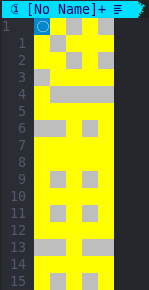
\includegraphics[
    width = 0.3\linewidth,
  ]{dotfont}
  \caption{点阵字模}%
  \label{fig:dotfont}
\end{figure}

\subsubsection{红外遥控}%
\label{ssub:ir}

原理和键盘扫描相同。用轮询法即可。只是从有线连接变成了无线连接。

\end{document}

